% !TEX root=/home/tavant/these/manuscript/src/manuscript.tex

\section{Instability in the \acs{2D} radial-azimuthal \acs{PIC} simulations}
  \label{sec-PIC-ECDI}
  
  \subsection{Introduction and state of the art} \label{subsec-indroECDI}
        
    The presence of azimuthal instabilities in the Hall effect thrusters has first been shown with numerical simulations by \citet{adam2004}.
    Then, they have been the subject of numerous studies, especially numerical \citep{ducrocq2006,lafleur2016,lafleur2016a,croes2017,croes2018,janhunen2018,taccogna2019}, but also experimental \citep{honore2011,cavalier2013,cavalier2013a}.
    However, their nature remain unclear \citep{boeuf2018}.
    Viven Croes studied the azimuthal instability in a bi-dimensional (\acs{2D}) radial-azimuthal simulation domain of radial length $L_R=2\,\centi\meter$ and azimuthal length $L_{\theta}=0.5\,\centi\meter$, with the model of particle convection proposed by Lafleur \citep{croes2017,croes2018}.
    He showed that the saturation of the oscillations was due to ion-wave trapping.
    Using a parametric study over the plasma density and the ion mass, he observed that the main oscillation is consistent with the characteristics of the \ac{IAW}.
    
    During the three years of my Ph.D., other groups presented new simulation results in similar radial-azimuthal geometries.
    \citet{hara2019a} presented kinetic simulation results on a two-dimensional domain, of size similar to the case studied here.
    However, that work was focused on the electron mobility values, and little information on the instability is given.
    In \citet{janhunen2018}, the authors presented a collisionless highly resolved \acs{2D} \ac{PIC} simulation.
    No convection and no compensation model for radial losses are used, hence the electron energy quickly rises and the density decreases.
    On the other hand, the domain is bigger, with a radial length of $L_r = 53.8\,\milli\meter$ for an azimuthal length of $L_{\theta} = 13.45 \,\milli\meter$.
    Three cells by Debye length are used, while there are on average 800 particles per cell.
    Under these conditions, the instability rises, but a large radial structure, named Modified Two Stream Instability (MTSI), of radial wavelength twice as big as $L_r$  is observed.
    The simulation parameters of \citet{taccogna2019} are similar to the results presented here, with  $L_r = 15\,\milli\meter$ and $L_{\theta} = 12.5 \,\milli\meter$.
    The results are qualitatively similar to the others, however the authors also observed radial structures, but this time with a wavelength of a third of $L_r$.
        
    \vspace{1ex}
    We can see that the results obtained with similar configurations differ significantly, meaning that some points needs to be clarified.
    % Therefore, we present in this chapter the results obtained with \LPPic.  
    In \cref{sec-PIC-ECDI}, we present the oscillations observed in the \ac{PIC} simulations carried out with \LPPic.
    After that, we derive the dispersion relation with no hypothesis concerning the particle distribution functions in \cref{sec-DR-kinetic}, and we present in \cref{sec-DR-solver} a numerical algorithm that solves the dispersion relation using the distribution function measured in the \ac{PIC} simulations.
    The oscillations observed in the simulation are compared in \cref{sec-DR-results} to the results of the dispersion relation.
    To finish with, the impact of the radial boundary condition is investigated in \cref{sec-DR-BC}.


  \subsection{Overview of the 2D simulation} \label{subsec-lppic_ECDI}
  
    
    We present in this section the simulation conducted to study the azimuthal instability.
    The parameters of the simulation are given in \cref{tab-evdfpicparams}.
    The imposed axial electric field $E_z$ and the radial magnetic field $B_r$ are uniform in space and constant in time.
    The radial direction is closed with the dielectric boundary condition of dielectric width $L_{diel}=3\,\milli\meter$.
    No \ac{SEE} is modeled, and the convection is modeled with the new noiseless model (see \cref{sec-noiselessresults}).
    The simulation is initialized with a uniform electron and ion density $n_e = n_i = \sn{3}{17}\per\meter\cubed$, with an electron temperature $\Te=10\,\volt$ and an ion temperature $\Ti=0.025\,\volt$.
    The mean particle density is conserved by imposing an ionization  which compensate the particle losses at the wall a each time step.
    
    \begin{table}[!hbt]
    \ra{1.3}
      \centering
      \caption{Parameters of the \acs{2D} \acs{PIC} simulations}
      \label{tab-evdfpicparams}
      \begin{tabular}{@{}r l l l @{}} \toprule
        {\bf Physical Parameter} &  &   &  \\
      Parameter                    & Symbol                          & Value                    & Unit \\ \midrule
      Dimensions                   & $L_r\times L_{\theta}\times L_z$ & $1\times 0.26\times 0.5$ & cm \\
      Radial magnetic field        & $B_r$                            & 0.02                     & T \\
      Axial electric field         & $E_z$                            & \sn{2}{4}                & $s\volt\per\meter$ \\
      Dielectric layer of width    & $L_{diel}$                       & 3                        & \milli\meter \\
      Mean plasma density          & $n_{0}$                          & $3 \times 10^{17}$       & {m}$^{-3}$ \\
      Initial electron temperature & $\Te_{,0} $                      & $10.0$                   & V \\
      Initial ion temperature      & $\Ti_{,0} $                      & $0.025$                  & V \\
      Duration of the simulation   & $T_{\rm simu}$                   & $7$                      & $\micro\second$ \\
      \midrule
      {\bf Numerical Parameter}    &                                  &                          & \\
      Time step                    & $\Delta t $                      & $4 \times 10^{-12}$      & s \\
      Cell size                    & $\Delta x = \Delta y$            & $2 \times 10^{-5}$       & m \\
      Number of particles per cell & $N/NG $                          & $80$                     & part/cell \\
      \bottomrule
      \end{tabular}
    \end{table}
    
    \Cref{fig-profiles_ne_one} shows the radial profile of the electron and ion densities, as well as the plasma potential, at the end of the simulation, averaged azimuthally and in time between $t=4$ and $7\,\micro\second$.
    The results are averaged azimuthally and in time over the 3 last microseconds.
    We can observe on the radial profile of both the densities and the plasma potential the sheaths close to the walls (regions of high electric field due to a charge unbalance) and the quasineutral plasma bulk in the center.
    These profiles are typical of low temperature low pressure bounded plasmas.
    
    \begin{figure}[hbt]
      \centering
      \begin{tabular}{@{} cc @{}}
        \subfigure{Ch5_radial_profiles}{a}{20, 15}
            &
        \subfigure{Ch5_radial_profiles_phi}{b}{20, 15} \\

      \end{tabular}
      \caption{Radial profile of ({\bf a}) the ion and electron densities, and ({\bf b}) the plasma potential, averaged azimuthally and in time between $t=4$ and $7\,\micro\second$.}
      \label{fig-profiles_ne_one}
    \end{figure}

    \Cref{fig-canon_Te_allch5} shows the temporal evolution of the mean kinetic energy $\Ee$ during the simulations.
    The mean kinetic energy is computed in the simulations by averaging over the whole electron population
    \begin{equation} \label{eq-Ee}
      \Ee_d = \frac{m_e}{2 e N_e} \sum_{j=1}^{N_e} v_{j, d}^2 
    \end{equation}
    with $d$ the direction ($r,\theta$, or $z$), $N_e$ is the number of electrons, and $v_{j, d}$ is the velocity in the direction $d$ of the $j^{\rm nt}$ electron.
    We see that the simulation starts at $\Ee = \Te_{,0} /2$, and  that after a few microseconds of transition, the simulations reaches a quasi steady-state with small fluctuations, that we name the saturated regime.
    This corresponds to an initial Debye length of $\lde=\sn{4.3}{-5}\,\meter$, increasing up to  $\lde=\sn{7.0}{-5}\,\meter$ during the saturated regime.
    \begin{figure}[!hbt]
      \centering
      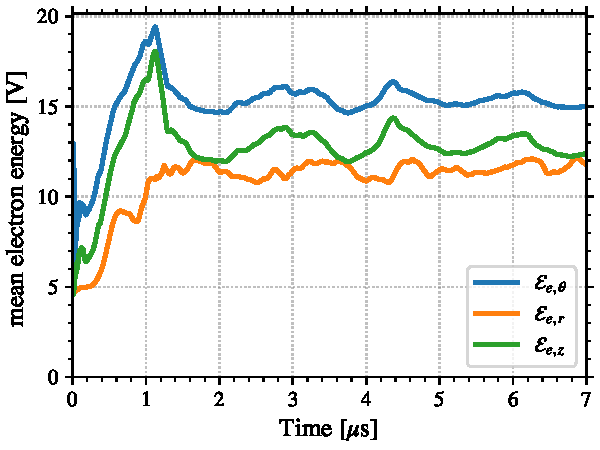
\includegraphics[width=\defaultwidth]{canonical_Te_all_directions.pdf}
      \caption{Temporal evolution of $\Ee$ the electron mean kinetic energy decomposed  over the three directions. The kinetic energy includes the internal energy (temperature) and the kinetic energy of the mean velocity.}
      \label{fig-canon_Te_allch5}
    \end{figure}
    

  \subsection{General characteristics of the azimuthal instability }
    In this section, we present the general characteristics of the azimuthal instability observed in the \ac{2D} \ac{PIC} simulations.
    \Cref{fig-2D_ne} shows the radial-azimuthal distribution of the electron density and the plasma potential during the saturated regime.
    We can see the instability in the azimuthal direction with a wavelength of a third of the azimuthal length.
    The instability can be seen in all of the plasma quantities (electron and ion densities, potential, electric field).
    In the radial direction, we can see the presheaths and the sheaths, characterized by the decrease of the plasma density between the center and the walls.

    \begin{figure}[hbtp]
      \centering
      % 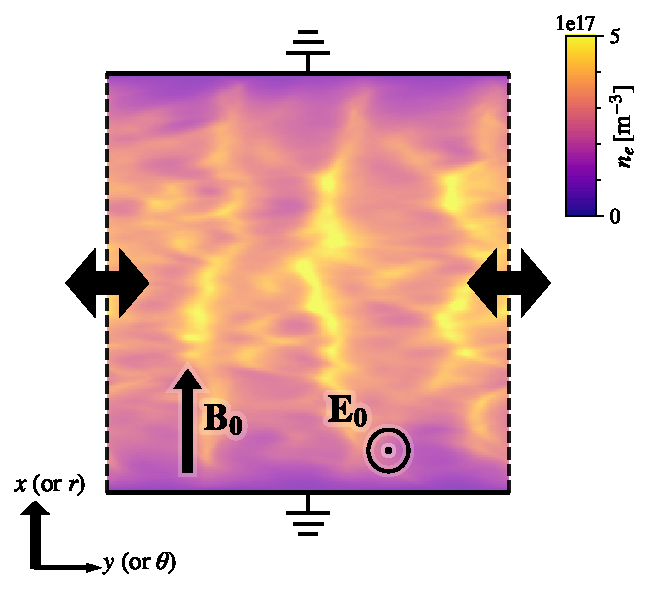
\includegraphics[width=\defaultwidth]{2D_schema_ne}
      \begin{tabular}{@{} c c @{}}
        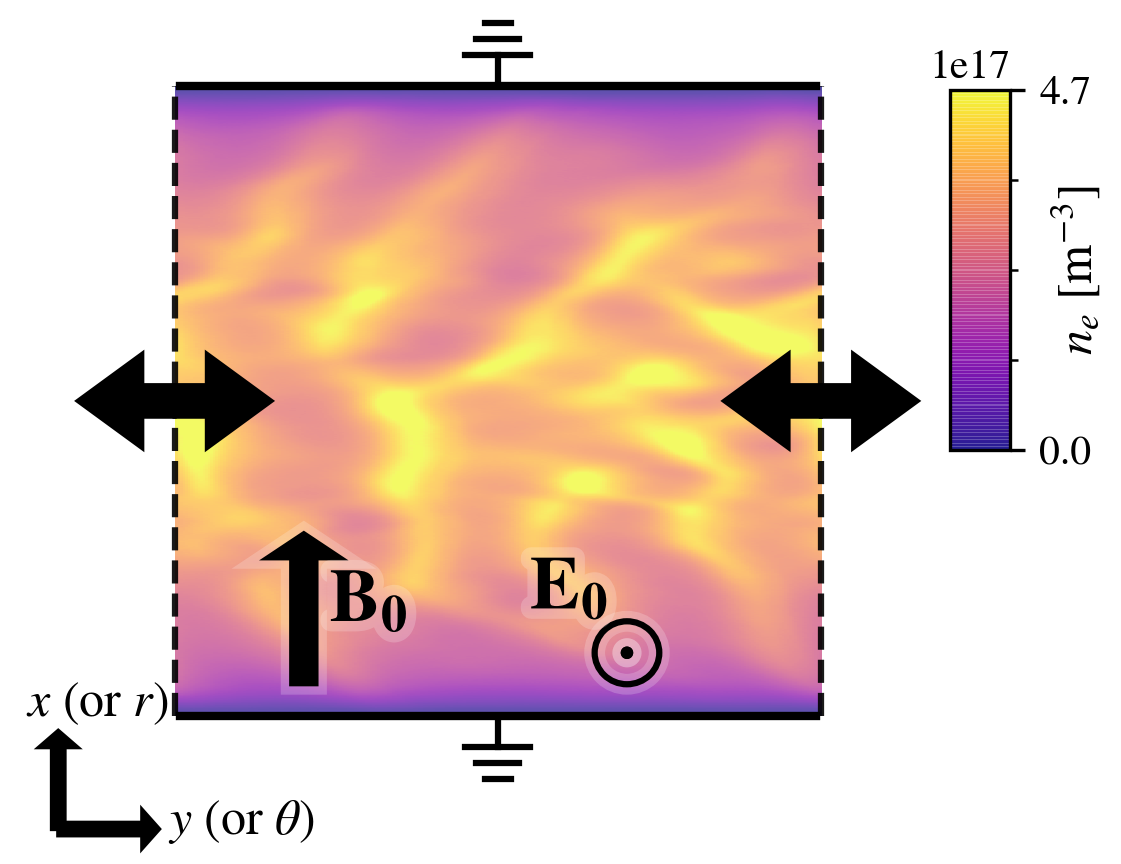
\includegraphics[width=0.485\textwidth]{2D_ne_ch5} &
        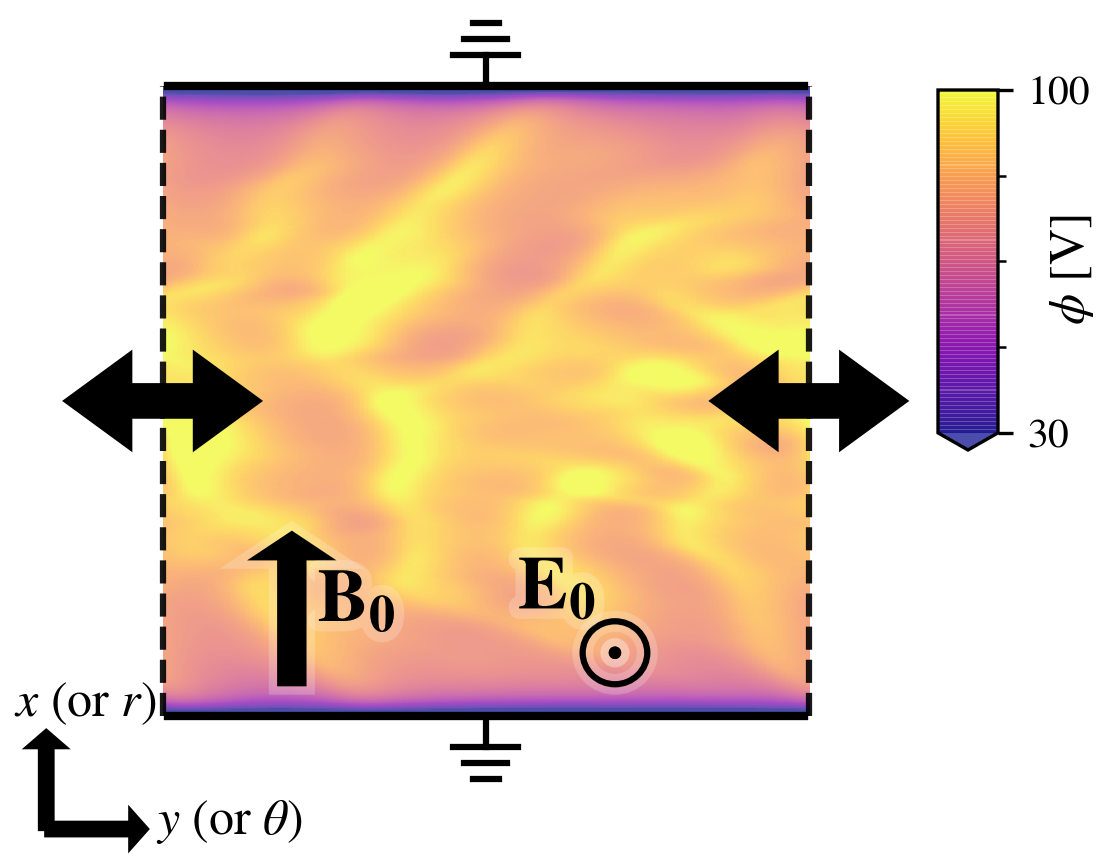
\includegraphics[width=0.485\textwidth]{2D_phi_ch5} \\
      \end{tabular}
      \caption{Radial and azimuthal distribution of (left) the electron density $n_e$ at $t=6\,\micro\second$ (during the saturated regime), and (right) the plasma potential $\phi$. The azimuthal instability is clearly seen, as well as the sheaths in the radial direction. }
      \label{fig-2D_ne}
    \end{figure}
    
    \Cref{fig-2DcutEx} shows the temporal evolution of the azimuthal electric field and the electron density as a function of the azimuthal position, measured at the center of the radial direction.
    We see the instability growing at the beginning, up to the saturation around $t=1\,\micro\second$.
    Then, we observe, in addition to the fast oscillation, a slower modulation of the oscillation amplitude, similar to the fluctuations seen in \cref{fig-canon_Te_allch5}.
    \begin{figure}[!hbt]
      \centering
      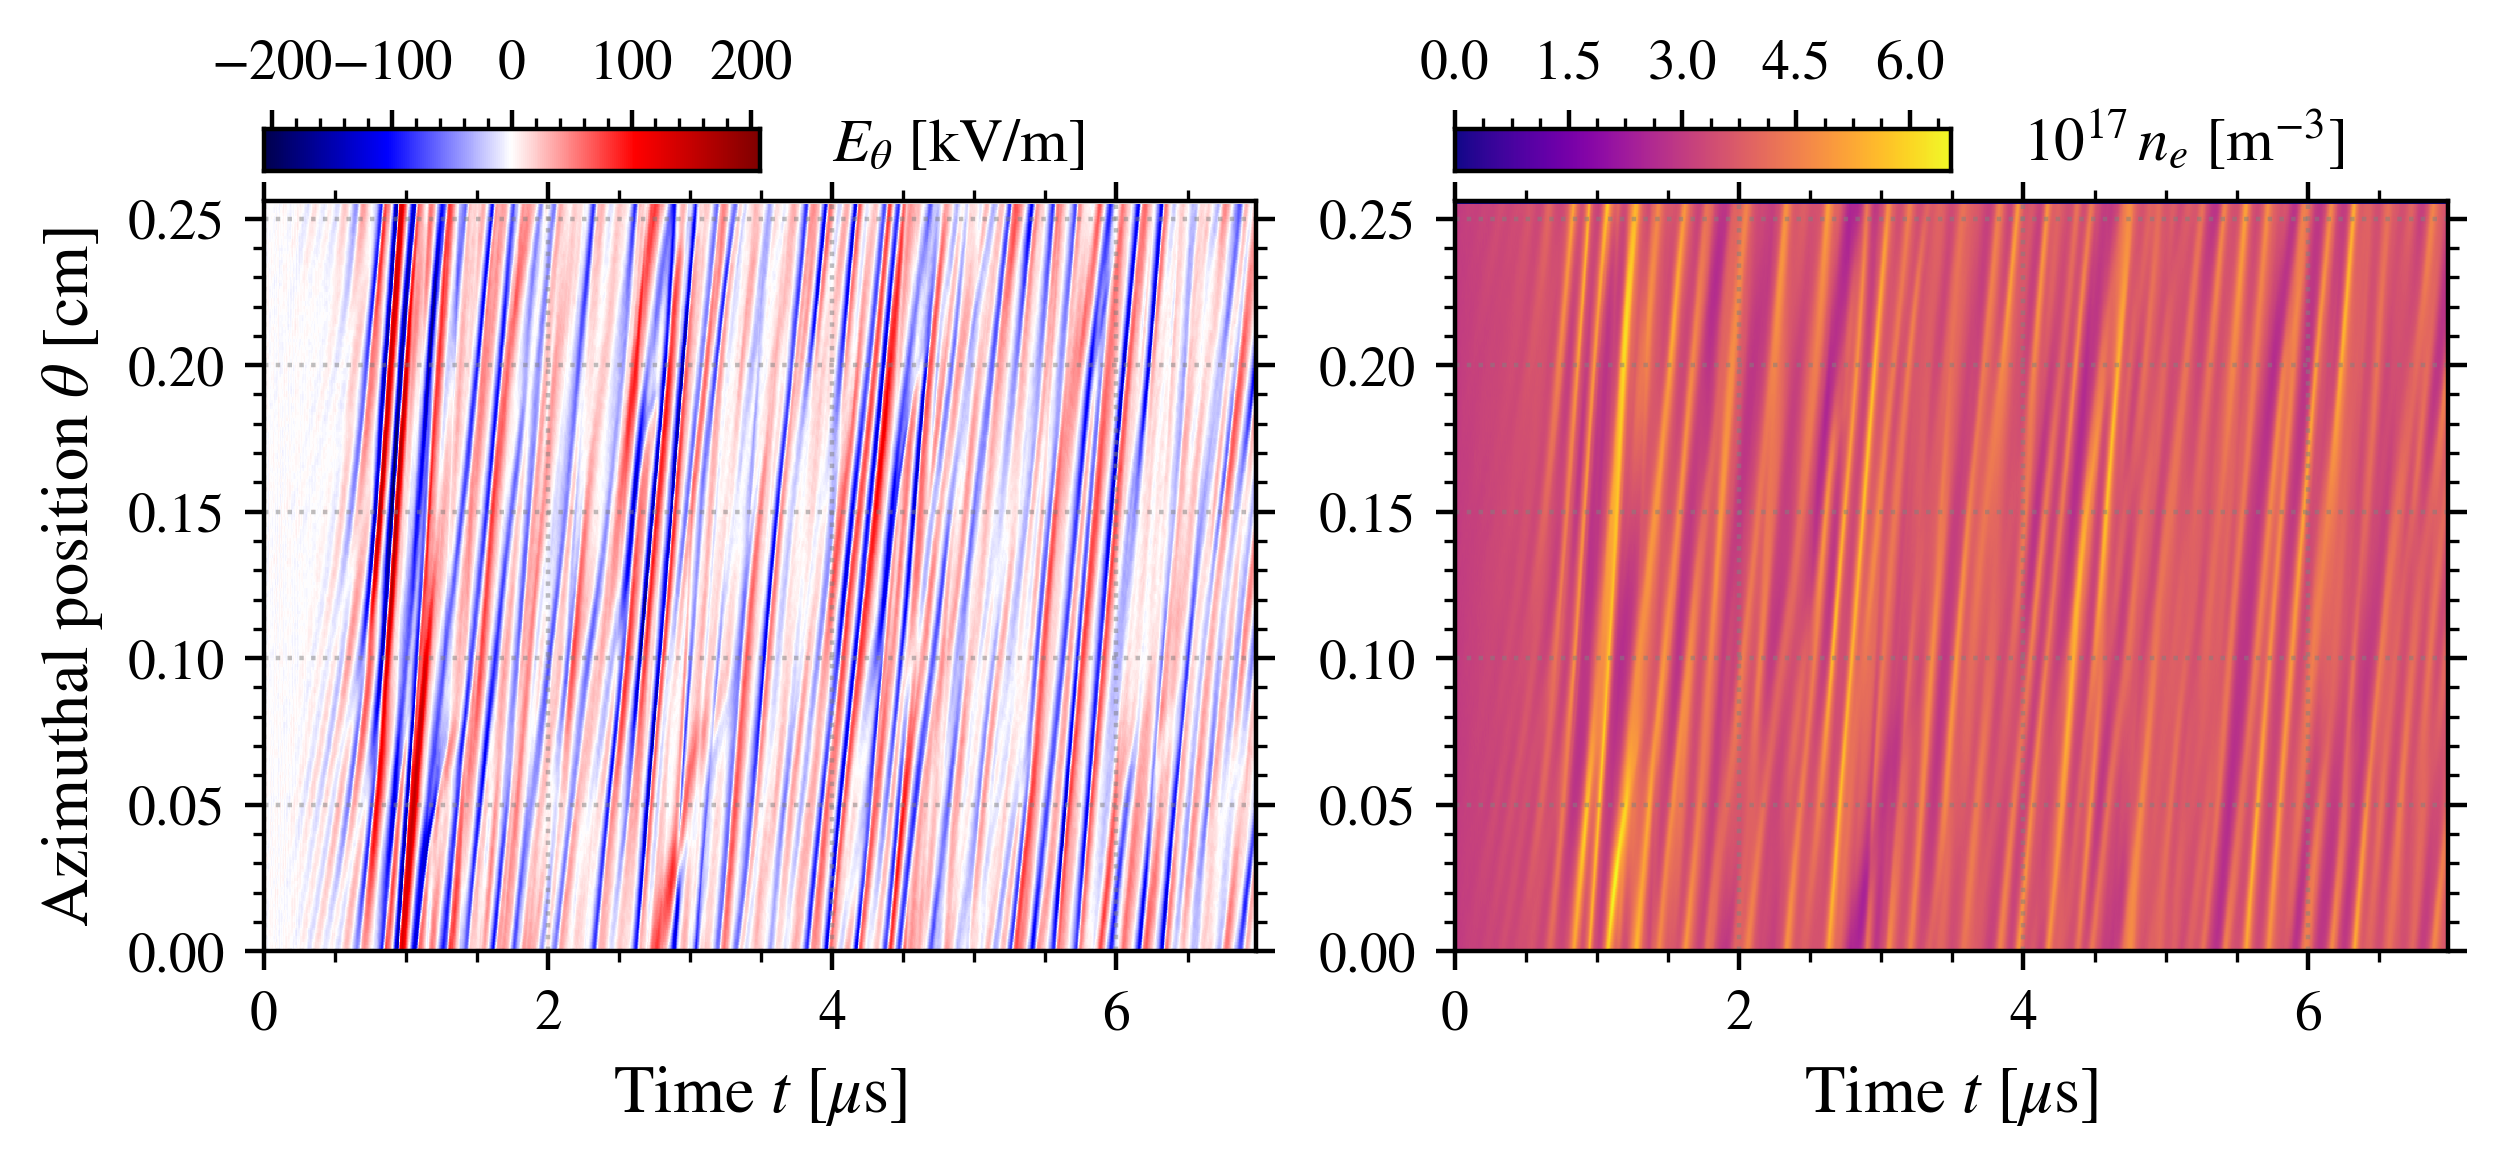
\includegraphics[width=\textwidth]{R_theta_fluctuations}
      \caption{Temporal evolution of (left) the azimuthal electric field $E_{\theta}$, and (right) the electron density $n_e$ as a function of the azimuthal position.}
      \label{fig-2DcutEx}
    \end{figure}

    \Cref{fig-FFT_ex} shows the frequency spectrum of the azimuthal electric field presented in \cref{fig-2DcutEx} computed via \ac{FFT} in the saturated regime between $2$ and $7\,\micro\second$.
    The spectrum has been averaged in the azimuthal direction, in order to reduce the noise.
    The theoretical frequency $f_{\rm theo} = \frac{\opi}{\pi \sqrt{6} }$ \citep{croes2018} is shown with a dashed line. 
    We can see a very good agreement between $f_{\rm theo}$ and the maximum of the frequency spectrum.
    The value of the theoretical frequency $f_{\rm theo}$ corresponds to the most growing frequency of the \ac{IAW} and is detailed in \cref{sec-DR-kinetic}.
    \begin{figure}[!hbt]
      \centering
      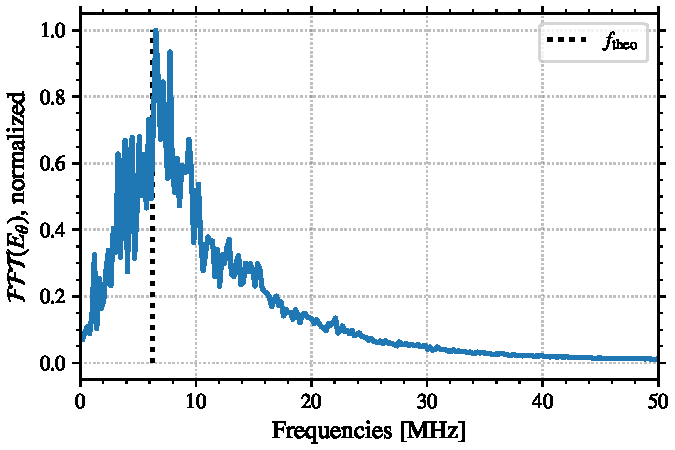
\includegraphics[width=\defaultwidth]{spectrum_frequency}
      \caption{Frequency spectrum of the azimuthal electric field computed between $2$ and $7\,\micro\second$, averaged in the azimuthal direction. The black line is the theoretical frequency $f_{\rm theo} = \frac{\opi}{\pi \sqrt{6} }$.}
      \label{fig-FFT_ex}
    \end{figure}
    
  \subsection{Energy cascade} \label{subsec-turbul}
  
    We can see in \cref{fig-FFT_ex} a slow decrease of the frequency amplitude from $f_{\rm theo}$ to larger frequencies.
    This type of cascade may be the signature of turbulence, and can be a source of energy dissipation - hence saturation.
    Kolmogorov's hypothesis of incompressible fluid leads to a cascade in power law \[ W(f) = | \mathcal{FFT}(E_{\theta})(f) |^2 \propto f ^ {- \alpha}, \]
    with $\alpha = 5/3$.
    \begin{figure}[!hbt]
      \centering
      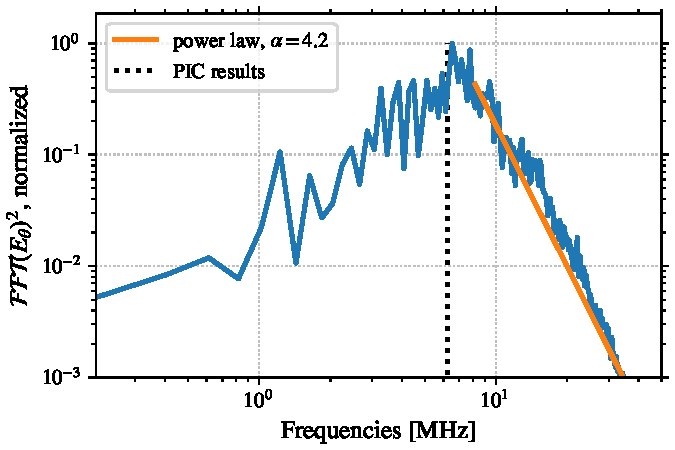
\includegraphics[width=\defaultwidth]{spectrum_frequency_turbul}
      \caption{Normalized frequency power spectrum in log-log scale computed between $1.5$ and $7\,\micro\second$. The black dotted line shows the  theoretical frequency $f_{\rm theo}$, the orange solid line is a linear fit of coefficient $\alpha$, and the green dashed line correspond to Kolmogorov's turbulent spectra. }
      \label{fig-turbul}
    \end{figure}
    
    \Cref{fig-turbul} shows the frequency power spectrum computed between $2$ and $7\,\micro\second$ in log scale.
    Overlaid is a fit of the cascade, for frequencies above the maximum amplitude.
    The power law obtained is $\alpha \simeq 4.2$, which is much greater than Kolmogorov's value of $5/3$.
    The oscillations observed present a decrease of the power spectrum much steeper than expected from turbulence.
    Even if the mechanism of plasma turbulence differs from the fluid turbulence \citep{tsytovich1972}, the value of $\alpha$ is significantly larger than expected.
    Consequently, we expected that there is no significant dissipation or cascade to the small scales.
  
  \subsection{Temporal evolution of the oscillation amplitude} \label{subsec-temp}
    We have seen in the previous section that after a growing phase, the amplitude of the instability saturates with a low frequency oscillation around a stable value.
    This section analyses these temporal characteristics.
    
    \Cref{fig-Ezstd_time} shows the temporal evolution of the characteristics of the electrostatic oscillation.
    As the oscillation is not monochromatic (i.e. it is the sum of multiple waves), we display both the maximum of the electric field $\max(E_{\theta})$, and its standard deviation $\stdE$.
    In the case of a monochromatic wave, one would have 
    \[ \stdE = \frac{\max(E_{\theta})}{\sqrt{2}}.  \]
    
    \begin{figure}[!hbt]
      \centering
      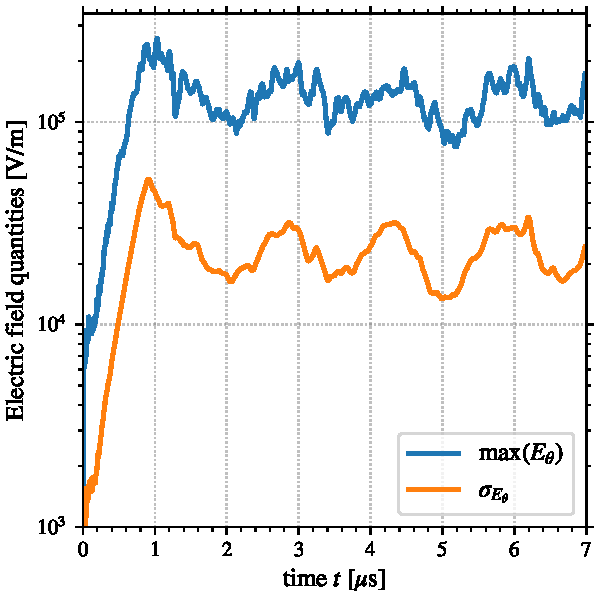
\includegraphics[width=\defaultwidth]{Temporal_E_theta.pdf}
      \caption{Temporal evolution of the maximum and the standard deviation of the azimuthal electric field, in log scale.}
      \label{fig-Ezstd_time}
    \end{figure}
    
    We can see in \cref{fig-Ezstd_time} that during the first microsecond, the growth of the wave amplitude is exponential, corresponding to a constant growth rate $\gamma_{PIC}$ that can be extracted from the simulation.
    A linear fit in log scale give $\gamma_{PIC} \simeq 0.07 \opi$ during the linear phase.
    After $t=1\,\micro\second$, the amplitude of the electric field oscillates around a mean value, with a period of the order of $T_{NL}=1.5 \pm 0.1 \,\micro\second$ ($NL$ for {\it non-linear} oscillation).
    Hence, the azimuthal electric field becomes of the type of
    \[  E_{\theta} = E_{\rm LF}(t) E_{\rm HF}(t, {\theta}) \]
    with $E_{\rm HF}(t, \theta) $ the high frequency instability, and $E_{\rm LF}(t)$ the low frequency modulation of the amplitude, with a low frequency $f_{\rm LF} \simeq  660 \pm 45 \,\kilo\hertz$.
    Several phenomena are candidates to the modulation observed, which are discussed here-after.
    
  
  \paragraph{Ion transit time\\}
    The ions are injected at the anode, and are accelerated by the uniform axial electric field $E_z$.
    The transit time of the ions in the axial direction $T_t$  is the time needed for the ions to travel $L_z$. Neglecting the collisions we have
    \begin{equation} \label{eq-transittime}
      T_{t} = \sqrt{\frac{2 m_i L_z}{e E_z}} \simeq 0.8 \mu s.
    \end{equation}
    
    The transit time is of the good  order of magnitude, but $T_{NL}$ is still twice bigger.
    In addition, we tried to initialize the simulation with ions distributed in the axial direction, so that their flux is constant in time.
    Such an initialization did not modify the low frequency oscillations.
    
  \paragraph{Particle trapping and bouncing\\}
    A common reason for wave saturation is the ion-wave trapping.
    The ion-wave trapping is a particle wave interaction that happens for the ions that have a velocity near the phase velocity of the wave.
    Ions are first accelerated by the wave where the electric field is positive.
    Hence, their velocity become slightly above the phase velocity of the wave, so that they reach the negative electric field of the wave.
    Then, their decelerate and reaches the first step of the process. 
    
    Ion-wave trapping has been observed in both \ac{1D} simulation by \citet{lafleur2016a} and in \ac{2D} simulation \citep{croes2017a}.
    Hence, the low frequency modulation could be due to the ions bouncing \citep{belmont2013}.
    However, the bouncing time scale is 
    \begin{equation} \label{eq-TB}
      T_{B} = 2 \pi \sqrt{\frac{m_i}{e k \max(E_{\theta})} } \simeq 0.5 \,\micro\second,
    \end{equation}
    which is 3 times smaller than $T_{NL}$.
    Using $\sqrt{2} \sigma_{E_{\theta}}$ instead of $\max(E)$, we find $T_B = 0.9\,\micro\second$.
    Even though in \citet{belmont2013}, the authors say that when the amplitude of the electric field is large (as it is the case here), the bouncing time scale increases due to non-linear phenomenon (the particle trajectory is no longer harmonic), we cannot conclude for now that this is the origin of the low frequency modulation.

  
  \paragraph{Ion-wave trapping oscillation\\}
    The wave saturating due to ion-wave trapping has an amplitude of \citep{lafleur2017,boeuf2018}
     \begin{equation} \label{eq-iontropempl}
       \stdE = \frac{\Te}{12 \lde}.
     \end{equation}
    
    Defining the wave energy  density by
    \begin{equation} \label{eq-waveE}
      \epsilon_{\rm wave} = \frac{\epsilon_0}{2} \stdE^2
    \end{equation}
    and the electron thermal energy density with
    \begin{equation} \label{eq-thE}
      \epsilon_{\rm th} = \frac{3}{2} e n_e \Te
    \end{equation}
    
    Using \cref{eq-iontropempl} in the definition of the wave energy \cref{eq-waveE} and the definition of the Debye length $\lde$ \cref{eq-def_lde}, we obtain
    \begin{align*} \label{eq-step_1}
      \epsilon_{\rm wave} &=  \frac{\epsilon_0}{2} \frac{\Te^{(2)}}{12^2} \frac{e^2 n_e}{ \epsilon_0 e\Te}\\
      &= \frac{e n_e \Te }{288} = \frac{\epsilon_{\rm th}}{432}
    \end{align*}
    This gives us a criterion for the ion-wave trapping using the wave and thermal energies
    \begin{equation} \label{eq-criteriaIT}
      432 \epsilon_{\rm wave} = \epsilon_{\rm th}.
    \end{equation}
    
    \Cref{fig-tempITcrit} shows the temporal evolution of the electron thermal energy $\epsilon_{\rm th}$ and the wave energy density $\epsilon_{\rm wave}$, scaled by the factor 432.
    We can see that $\epsilon_{\rm th}$ is relatively constant.
    However, $\epsilon_{\rm wave}$  oscillates significantly, and passes regularly above and below $\epsilon_{\rm th}$.
    In order to understand the reason for this behavior, we can look at the evolution of the ion temperature.
    Indeed, the trapped ions gain energy, which increases the total ion temperature. 
    
    
    \begin{figure}[!hbt]
      \centering
      % 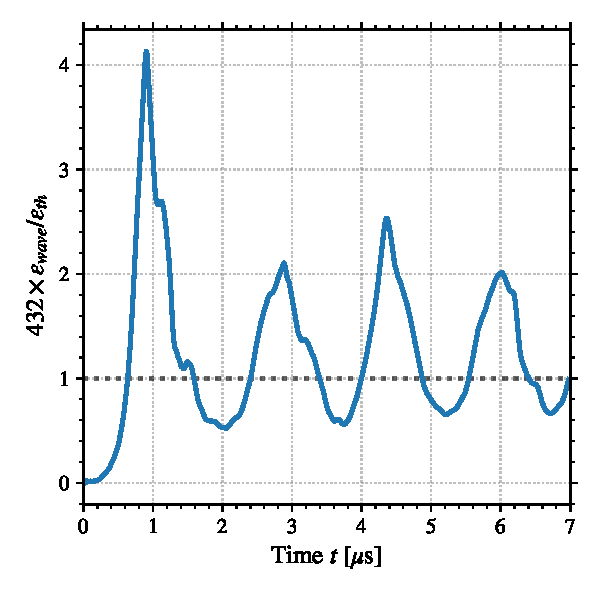
\includegraphics[width=\defaultwidth]{Ion_Trapping_criter}
      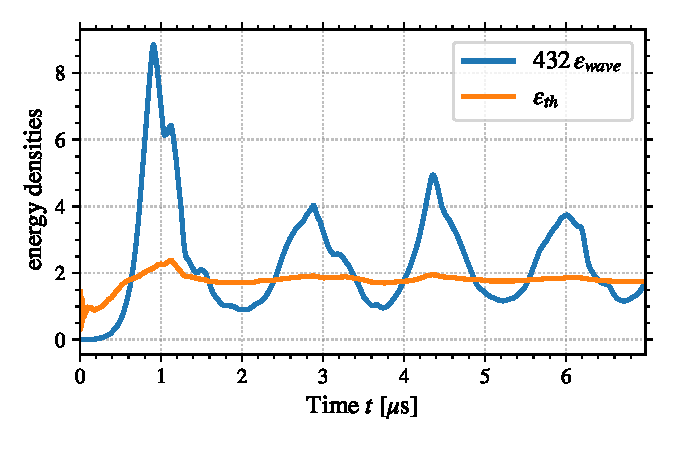
\includegraphics[width=\defaultwidth]{Ion_Trapping_criter_bis}
      \caption{Temporal evolution of the wave energy density $\epsilon_{\rm wave}$ compared to the thermal energy density $\epsilon_{\rm th}$.}
      \label{fig-tempITcrit}
    \end{figure}
    
    
    The correlation between the wave amplitude and the ion temperature is shown in \Cref{fig-oscillation_ion_cret}.
    \cref{fig-oscillation_ion_cret}.{\bf a} shows the temporal evolution of the ion temperature $\Ti$ and the standard deviation of the azimuthal electric field $\sigma_{E_{theta}}$, both normalized.
    We see that the oscillation of the wave amplitude is a quarter of a period before the oscillation of the ion temperature.
    This means that first the wave increases, then the ion temperature increases.
    After that, the wave amplitude decreases, which leads to the decreases of the ion temperature.
    
    \begin{figure}[!hbt]
      \centering
        \begin{tabular}{cc}
          \subfigure{Instability_amp_and_Ti}{a}{30,20} & 
          \subfigure{Instability_criterion_and_gradTi}{b}{20,20} \\
          
        \end{tabular}
        \caption{Temporal evolution of ({\bf a}) the ion temperature $\Ti$ and the standard deviation of the $\sigma_{E_{\theta}}$, normalized, and ({\bf b}) the temporal derivative of the ion temperature $\partial{\Ti}/\partial t$ and the ion-wave trapping criterion, normalized.}
      \label{fig-oscillation_ion_cret}
    \end{figure}
    
    \cref{fig-oscillation_ion_cret}.{\bf b} shows the temporal derivative of the ion temperature $\partial_t \Ti$ and the ion-wave trapping criterion defined as $432\epsilon_{\rm wave} - \epsilon_{\rm th}$ from \cref{eq-criteriaIT}, both normalized.
    When the ion-wave trapping criterion is negative, it means that the wave amplitude is too small, so that the ions are not trapped.
    In contrast, if it is positive the ions will be trapped.
    Again, we see a good correlation between the sign of the ion-wave trapping criteria and the growth, or decrease, of the ion temperature.
    
    In \cref{fig-tempITcrit,fig-oscillation_ion_cret}, the period of the oscillations of $\epsilon_{\rm wave}$ is $T_{NL} \simeq 1.5\,\micro\second$.
    This period could be related to the response time of the ions, as we have \citep{weiland1977} $$T_{NL}/4 \simeq 0.4\,\micro\second \sim T_B.$$
    The hypothesis that the low frequency modulation of the amplitude of the azimuthal wave could be validated by varying the ion mass, and observe if $T_{NL}$ varies in $\sqrt{m_i}$.    
    To summarize, the low frequency modulation of the azimuthal wave amplitude is certainly due to non-linear behavior of wave-particle interaction.
    Complementary results are presented in \cref{subsec-VDFIAW} by solving the dispersion relations.
    
